%----------------------------------------
% SECTION: Toric Code and its features
%----------------------------------------
\section{Toric Code and its features}
\label{sec:toric_code_and_its_features}

The Toric code is two-dimensional model of spin-\onehalf degrees of freedom (d.o.f).
It can be regarded as an example of a pure $\mathbb{Z}_2$ lattice gauge theory.
In particular we focus on a $L \times L$ square lattice (with periodic boundary conditions), and the d.o.f.~are defined on the links the lattice.
The local Hilbert space is $\mathbb{C}^2$ and as a basis we can use the computation basis (or $Z$-basis) $\qty{ \ket{0}, \ket{1} }$ for which the Pauli matrix $\sigma^z$ (shortened as $Z$) is diagonal.
The main local operators (that enters the Hamiltonian) are defined on the \emph{stars} (the links attached to a given site) and \emph{plaquettes} (links around a face) of the lattice:
\begin{equation}
    A_v = \prod_{j \in \text{star}(s)} \sigma^z_j, \qquad
    B_p = \prod_{j \in \partial p} \sigma^x_j.
\end{equation}
One can easily prove the following commutation relations of the $A_s$s and $B_p$s operators
\begin{equation}
    [ A_v, A_{v^{\prime} } ] = 0, \quad
    [ B_p, B_{p^{\prime} } ] = 0, \quad
    [ A_v, B_p ] = 0
    \label{eq:star_plaq_op_comm}
\end{equation}
for all $v$, $v^{\prime} $ and $p$, $p^{\prime} $.
The eigenvalues of the Pauli matrices are just $pm 1$, so the same holds true for $A_s$ and $B_p$.
Moreover, like the Pauli matrices, also $A_s^2 = \One$ and $B_p^2 = \One$.


Now, we proceed with writing the Toric Code Hamiltonian:
\begin{equation}
    H = - \sum_{v} A_v - \sum_{p} B_p
    \label{eq:toric_code_hamiltonian}
\end{equation}
which is \emph{exactly solvable}.
Indeed, given \eqref{eq:star_plaq_op_comm}, one can find a ground state $\ket{\Omega}$  by simply imposing a set of constraints
\begin{equation}
    A_v \ket{\Omega} = \ket{\Omega}, \qquad
    B_p \ket{\Omega} = \ket{\Omega}, \qquad \forall v,
    \label{eq:ground_state_constraints}
\end{equation}
Even more, it is possible to define the set of ground states
\begin{equation}
    \mathcal{L} = \qty{ \ket{\Omega} : A_s \ket{\Omega} = \ket{\Omega}, \quad B_p \ket{\Omega} = \ket{\Omega} \quad \forall s, p }
\end{equation}
which contents \emph{depends on the topology of the lattice}.
For example, if the lattice has periodic boundary conditions, then there are $4$ degenerate ground states $\ket{\Omega_{u,v}}$ with $u, v = \pm 1$, which can be distinguished only by non-local operators.
We will see how later.

\begin{figure}[t]
    \centering
    \begin{tikzpicture}[
        scale=1.2,
        site/.style = {circle, inner sep=0 pt, minimum size=3pt, draw=black, fill=white},
        plaq/.style={blue, ultra thick},
        gauss/.style={red, ultra thick}
        ]
    % Lattice
    \draw[thin] (-0.5,-0.5) grid (4.5,2.5);

    % Plaquette operator
    \draw[plaq] (3,1) -- (4,1) node [pos=0.5, below] {$X$};
    \draw[plaq] (4,1) -- (4,2) node [pos=0.5, right] {$X$};
    \draw[plaq] (4,2) -- (3,2) node [pos=0.5, above] {$X$};
    \draw[plaq] (3,2) -- (3,1) node [pos=0.5, left]  {$X$};
    \draw[blue, ultra thick, pattern=north east lines, pattern color=blue] (3,1) rectangle (4,2);
    \draw (3.5,1.5) node [fill=white, rounded corners] {$B_p$};

    % Gauss operator
    \draw[gauss] (1, 1) -- (2, 1) node [pos=0.5, below right] {$Z$};
    \draw[gauss] (1, 1) -- (1, 2) node [pos=0.5, above left] {$Z$};
    \draw[gauss] (1, 1) -- (0, 1) node [pos=0.5, below left] {$Z$};
    \draw[gauss] (1, 1) -- (1, 0) node [pos=0.5, below right] {$Z$};

    \foreach \y in {0,1,2} \foreach \x in {0,1,...,4} \draw (\x,\y) node [site] {};

    \draw (1,1) node [above right, outer sep=5pt, inner sep=3pt, draw=red, rounded corners=3pt] {$A_s$};
\end{tikzpicture}

    \caption{Graphical representation of the Toric Code operators $A_s$ and $B_p$}
\end{figure}

\subsection{Ground states}
\label{sub:ground_states}


Consider a torus geometry for the lattice, i.e.~periodic boundary conditions in both directions, of size $L \times L$.
From \eqref{eq:ground_state_constraints}, we have $2L^2$ constraints but these are not all independent.
In fact on a torus, one can see that
\begin{equation}
    \prod_{v} A_{v} = \One, \qquad
    \prod_{p} B_p = \One
\end{equation}
which actually means that there are $2L^2 - 2$ independent conditions.
The total Hilbert space has dimension $2^{2L^2}$, therefore the space $\mathcal{L}$ has dimension $2^{2L^2 - 2L^2 + 2} = 4$, which means that the Toric Code has $4$ degenerate ground states.
These states all satisfy the same set \eqref{eq:ground_state_constraints} of equations, which means that they\emph{cannot be distinguished by local operators}.
This is typical of topological phases in two dimensions \todo{ref}.

These ground states can only be distinguished by non-local operators that have to commute with Hamiltonian in \eqref{eq:toric_code_hamiltonian}, hence with all $A_v$ and $B_p$ but cannot be expressed in terms of $A_v$ and $B_p$.
The only operators that satisfy this requirements are defined on closed paths, on the direct or dual lattice, that cannot be reduced to a single plaquette loop (on the dual lattice the plaquettes are the stars of the direct lattice).
In other words, they are defined along \emph{non-contractible loops}.
The reason being that any product of $\sigma^x$ or $\sigma^z$ along a closed curve $\mathcal{C}$ that commutes with the Hamiltonian can be expressed as product of $A_v$ or $B_p$ of the stars or plaquettes enclosed by $\mathcal{C}$.
Consider now, two non-contractible curves $\mathcal{C}_{1}$ and $\mathcal{C}_{2}$ along the $\hat{1}$ and $\hat{2}$ direction respectively.
On these paths we can define the \emph{string operators}
\begin{equation}
    \overline{X}_1 = \prod_{j \in \mathcal{C}_1}  \sigma^x_j, \qquad
    \overline{X}_2 = \prod_{j \in \mathcal{C}_2}  \sigma^x_j,
    \label{eq:nonlocal_X_operators}
\end{equation}
it can be proved that they commute with all the local operators but cannot be expressed as a product of them.
The same can be repeated on the dual lattice, by considering dual non-contractible paths $\tilde{\mathcal{C}}_1$ and $\tilde{\mathcal{C}}_2$ and defining
\begin{equation}
    \overline{Z}_1 = \prod_{j \in \mathcal{\tilde{C}}_1}, \qquad
    \overline{Z}_2 = \prod_{j \in \mathcal{\tilde{C}}_2}
    \label{eq:nonlocal_Z_operators}
\end{equation}
Likewise, the operators in \eqref{eq:nonlocal_Z_operators} commutes with all the vertex and plaquettes operators but they do not commute with the X-operators in \eqref{eq:nonlocal_X_operators}.

In fact, \eqref{eq:nonlocal_X_operators} and \eqref{eq:nonlocal_Z_operators} have the same (anti)commutation relations of two qubits:
\begin{equation}
    \qty{ \overline{X}_1, \overline{Z}_2 } = 0, \qquad
    \qty{ \overline{X}_2, \overline{Z}_1 } = 0,
\end{equation}
Therefore, the Toric Code (on a torus) has a protected subspace $\mathcal{L}$ (the space of the ground states) that behaves like the Hilbert space of two qubits and the operators \eqref{eq:nonlocal_X_operators} and \eqref{eq:nonlocal_Z_operators} acts like unitary gates on this space.

\begin{figure}[t]
    \centering
    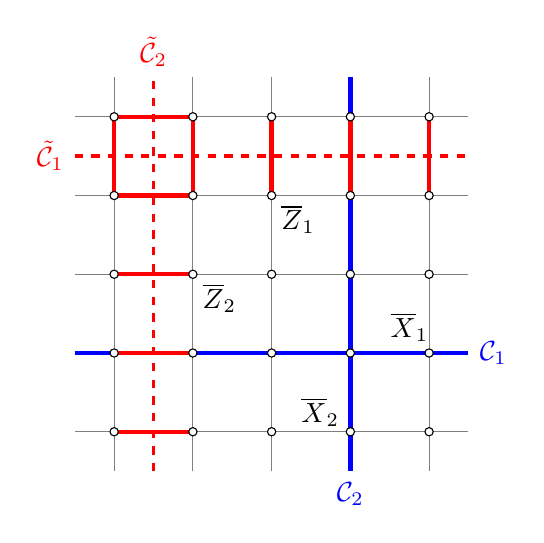
\begin{tikzpicture}[
        site/.style = {circle, inner sep=0 pt, minimum size=3pt, draw=black, fill=white},
    ]
    % lattice grid
    \draw[Gray,thin] (-0.5,-0.5) grid (4.5,4.5);

    % Wilson loops
    \draw[Blue, ultra thick]
        (-0.5, 1) -- (4.5, 1)
        node [pos=1, right] {$\mathcal{C}_1$}
        node [pos=0.85, above, black] {$\overline{X}_1$}
        ;
    \draw[Blue, ultra thick]
        (3, -0.5) -- (3, 4.5)
        node [pos=0, below] {$\mathcal{C}_2$}
        node [pos=0.15, left, black] {$\overline{X}_2$}
        ;

    % 't Hooft strings
    \draw[Red, very thick, dashed]
        (-0.5,3.5) -- (4.5,3.5)
        node[pos=0, left] {$\tilde{\mathcal{C}}_1$}
        ;
    \foreach \x in {0,...,4} { \draw[Red, ultra thick] (\x, 3) -- +(0, 1); }
    \draw (2,3) node [below right] {$\overline{Z}_1$};
    \draw[Red, very thick, dashed]
        (0.5,-0.5) -- (0.5,4.5)
        node[pos=1, above] {$\tilde{\mathcal{C}}_2$}
        ;
    \foreach \y in {0,...,4} { \draw[Red, ultra thick] (0, \y) -- +(1, 0); }
    \draw (1,2) node [below right] {$\overline{Z}_2$};
    \foreach \y in {0,...,4} \foreach \x in {0,...,4} \draw (\x,\y) node [site] {};
\end{tikzpicture}

    \caption{Non-contractible paths}
\end{figure}

\todo{revisionare}



\subsection{Particle excitations}%
\label{sub:particle_excitations}

Until now we have only discussed the ground states of the Toric Code, without touching the rest of the low energy sectors.
In other words, how do we describe the excitations of this model?
As we said, \eqref{eq:ground_state_constraints} are the set of constraints that defines the ground states.
Therefore, everytime a given state $\ket{\Psi}$ violates these equations, we will say that it contains \emph{particles}, which can be of different types.
If $A_v \ket{\Psi} = - \ket{\Psi}$, then we will say that the vertex $v$ contains a $z$-type particle.
Likewise, if $B_p \ket{\Psi} = - \ket{\Psi}$, then the plaquette $p$ contains a $x$-type particle.

Now the question: starting from a ground state $\ket{\Omega}$, how can we introduce some particles?
The answer is \emph{string operators}.
We are not considering closed strings, like we did in Sec.~\ref{sub:ground_states}, but any open string.
The shortest open string that we can consider is a single link.
So a $Z$-string on a single link is just $Z_j$, where $j$ is a label of a generic link.
Consider now the state
\begin{equation}
    \ket*{\Psi^Z} = Z_j \ket{\Omega},
\end{equation}
This state hosts particles at the ``boundaries'' of the $j$-th link, i.e.~the vertices touching $j$ which we call $v_0$ and $v_1$.
This can be proved by simply showing that $[ A_v, Z_j ] = 0$ for $v \neq v_0$ and $v \neq v_1$ and $\{ A_{v_0}, Z_j \} = \{ A_{v_1}, Z_j \} = 0$.
Which immediately implies that
\begin{equation}
    A_{v_0} \ket*{\Psi^Z} = A_{v_1} \ket*{\Psi^Z} = - \ket*{\Psi^Z}
\end{equation}

